\documentclass{article}

\usepackage[dblblindworkshop]{neurips_2026}
\workshoptitle{AXIOM 2026: Foundations of Efficient Deep Learning}

\usepackage[utf8]{inputenc}
\usepackage[T1]{fontenc}
\usepackage[hidelinks]{hyperref}
\usepackage{url}
\usepackage{booktabs}
\usepackage{amsmath,amssymb,amsfonts}
\usepackage{nicefrac}
\usepackage{microtype}
\usepackage{xcolor}
\usepackage{graphicx}
\usepackage{tikz}
\usepackage{seqsplit}
\usetikzlibrary{arrows.meta,positioning,fit}

\definecolor{pgblue}{RGB}{28,92,148}
\definecolor{pgorange}{RGB}{214,121,38}
\definecolor{pggreen}{RGB}{43,128,82}
\definecolor{pglight}{RGB}{235,242,249}
\definecolor{pgwarm}{RGB}{253,240,224}
\newcommand{\method}{PageGauge}
\newcommand{\Q}{\mathcal{Q}}
\newcommand{\E}{\mathcal{E}}

\title{PageGauge: Factoring Affine KV Quantization Through Softmax Attention}
\author{Anonymous Author(s)}

\begin{document}
\maketitle

\begin{abstract}
KV-cache quantization is usually designed as a storage format and then repaired
inside the attention kernel by fused elementwise reconstruction.  We instead
co-design the representation with the algebra of its consumer.  \method{} uses
token-independent channel centers and scalar page/head scales so key centers
cancel as a softmax-invariant shift, value centers are restored once, and page
scales become fragment-level corrections around FP16 code-valued contractions.
Exact FP16 regions compose with historical INT8 pages through online-softmax
state merging.  The transformation is exact in real arithmetic relative to the
reconstructed mixed-precision cache; quantization error remains separate.  On
Mistral-7B-v0.3 with a 20,480-token prefix, the fixed policy reduces B4 served-KV
storage by 36.86\% and rereads 48 runtime-appended pages through INT8.  Following
a disclosed TEST-visible precision-policy repair, six fixed-policy B1
WikiText-2 windows give minimum PageGauge/FP16 logit cosine 0.99871 and top-1
agreement 0.99891.  Eight order-balanced ABBA/BAAB fresh-process B4 blocks
measure 15.214 versus 17.232 ms per sustained complete-decoder step: a
1.1326$\times$ speedup (within-protocol hierarchical 95\% CI [1.1323, 1.1328]).
\end{abstract}

\section{Introduction}

Long-context autoregressive inference repeatedly streams a KV cache whose size
grows with sequence length.  Existing quantizers reduce storage, while fused
kernels hide reconstruction within attention \citep{liu2024kivi,hooper2024kvquant}.
This can still move affine metadata through the hottest contractions.  Our
starting axiom is broader: \emph{quantization should be co-designed with the
algebra and invariances of the operation that consumes the tensor}.  Softmax
attention is unusually favorable because it is invariant to a common key-logit
shift, normalizes value weights to one, and admits associative online-state
merging \citep{dao2022flashattention,dao2024flashattention2}.

KIVI and KVQuant primarily optimize low-bit cache representations
\citep{liu2024kivi,hooper2024kvquant}; BitDecoding and InnerQ coordinate
reconstruction with hardware execution \citep{du2025bitdecoding,hosseini2026innerq}.
HeadQ and OptR explicitly optimize attention-visible key geometry, including
equivalence modulo common logit shifts \citep{williams2026headq,yun2026optr},
while ScaleSearchAttention directly executes NVFP4 $QK/PV$
\citep{gupta2026scalesearch}.  PageGauge is complementary: it restricts affine
metadata so corrections factor around FP16 contractions in a paged decoder;
key centering itself is not claimed as new.

We make exactly three contributions.  (1) We give conditions under which the
center and scale metadata of pagewise affine K/V quantization factor outside
the main $QK$ and $PV$ code contractions.  (2) We realize this representation
in a FlashInfer-compatible decoder path that directly consumes historical
INT8 codes and merges them with exact FP16 regions without materializing a
reconstructed FP16 history.  (3) We validate explicit-reconstruction fidelity,
  predictive fidelity with runtime-appended-page recurrence, complete served-cache
  accounting, and repeated fresh-process complete-decoder speed against optimized FP16
FlashInfer \citep{ye2025flashinfer}.  We do not claim novelty for KV
quantization, exact recent windows, online softmax, or FlashInfer; the novelty
is the representation/kernel co-design that makes affine metadata factorizable.

\section{Attention-Compatible KV Quantization}

\subsection{Affine representation and proposition}

For one query/head, let $q\in\mathbb R^{1\times d}$,
$c_K,c_V\in\mathbb R^d$, $Z_p^K,Z_p^V\in\mathbb Z^{n_p\times d}$, and
$\mathbf1_p\in\mathbb R^{n_p}$.  Quantized page $p$ reconstructs as
\begin{equation}
 \widehat K_p=\mathbf1_pc_K^\top+s_p^KZ_p^K,\qquad
 \widehat V_p=\mathbf1_pc_V^\top+s_p^VZ_p^V,                 \label{eq:affine}
\end{equation}
where centers are shared over the complete attention domain and each scale is
scalar over one page/head tile.

\paragraph{Frozen quantizer.}
For $X\in\{K,V\}$ and initial-prefill length $L_0$, each request/layer/KV-head
uses
\begin{align}
c_X&=\operatorname{FP16}\!\left(L_0^{-1}\!\sum_{t=1}^{L_0}X_t\right),\nonumber\\
s_p^X&=\operatorname{FP16}\!\left[\max\!\left(2^{-20},
 \frac{\|X_p-\mathbf1_pc_X^\top\|_\infty}{127}\right)\right],\nonumber\\
Z_p^X&=\operatorname{clip}_{[-127,127]}\operatorname{round}_{\rm away}
 \!\left(\frac{X_p-\mathbf1_pc_X^\top}{s_p^X}\right).       \label{eq:quantizer}
\end{align}
The mean and max are computed in FP32; the stored FP16 scale is used in the
quotient, ties round away from zero, and centers are frozen and reused for all
runtime-appended pages.

\paragraph{Proposition 1 (factorized mixed-cache attention).}
Let $\Q$ index quantized pages and $\E$ the exact-token set, with
$K'_E=K_E-\mathbf1_Ec_K^\top$ and $V'_E=V_E-\mathbf1_Ec_V^\top$.  Define
$\widetilde K=\operatorname{concat}(\{s_p^KZ_p^K\}_{p\in\Q},K'_E)$ and
$\widetilde V=\operatorname{concat}(\{s_p^VZ_p^V\}_{p\in\Q},V'_E)$, so
$\widehat K=\mathbf1c_K^\top+\widetilde K$ and
$\widehat V=\mathbf1c_V^\top+\widetilde V$.  Then
\begin{equation}
 \operatorname{softmax}\!\left(\frac{q\widehat K^\top}{\sqrt d}\right)\widehat V
 =c_V^\top+\operatorname{softmax}\!\left(
 \frac{q\widetilde K^\top}{\sqrt d}\right)\widetilde V.    \label{eq:factorized}
\end{equation}
\emph{Proof.}  Since $q\widehat K^\top/\sqrt d=q\widetilde K^\top/\sqrt d+
(qc_K/\sqrt d)\mathbf1^\top$, softmax removes the global constant.  Let $P$
be that globally normalized row and $P_p,P_E$ its page/exact subvectors.  Then
\begin{equation}
 O=c_V^\top+\sum_{p\in\Q}s_p^VP_pZ_p^V+P_EV'_E,             \label{eq:value}
\end{equation}
because $P\mathbf1=1$.  Also
$q(s_p^KZ_p^K)^\top=s_p^Kq(Z_p^K)^\top$ and
$P_p(s_p^VZ_p^V)=(s_p^VP_p)Z_p^V$.  Thus scalar metadata is applied around the
code contractions at fragment granularity without materializing historical
elementwise reconstruction. $\square$  Full failure conditions are in Appendix~A.

\subsection{Mixed exact/quantized attention}

For segment $j$, centered scores and values $a_{j,i},\widetilde v_{j,i}$ define
$m_j=\max_i a_{j,i}$, $\ell_j=\sum_i e^{a_{j,i}-m_j}$, and
$o_j=\sum_i e^{a_{j,i}-m_j}\widetilde v_{j,i}$.  Their associative merge is
\begin{equation}
 m=\max_jm_j,\quad \ell=\sum_j e^{m_j-m}\ell_j,\quad
 o=\sum_j e^{m_j-m}o_j,\qquad O=o/\ell+c_V^\top.            \label{eq:merge}
\end{equation}
Thus a key-center offset is neither dropped per segment nor counted twice, and
the value center is added only after global normalization.  Figure~\ref{fig:path}
contrasts reconstruction-first execution with the factorized path.

\begin{figure}[t]
\centering
\resizebox{0.99\linewidth}{!}{%
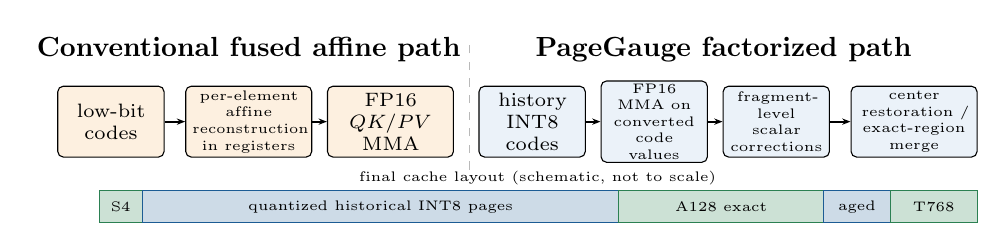
\begin{tikzpicture}[
  font=\scriptsize,
  box/.style={draw,rounded corners=2pt,minimum height=0.90cm,minimum width=1.35cm,
    text width=1.18cm,align=center,inner xsep=2pt,inner ysep=1pt},
  wide/.style={box,minimum width=1.60cm,text width=1.43cm},
  arr/.style={-{Stealth[length=3pt]},thick},
  note/.style={font=\tiny,align=center}
]
  \node[font=\bfseries] at (2.05,2.48) {Conventional fused affine path};
  \node[box,fill=pgwarm] (cq) at (0.30,1.56) {low-bit\\codes};
  \node[wide,fill=pgwarm,font=\tiny] (cr) at (2.05,1.56) {per-element affine\\reconstruction in registers};
  \node[wide,fill=pgwarm] (ca) at (3.85,1.56) {FP16 $QK/PV$\\MMA};
  \draw[arr] (cq)--(cr); \draw[arr] (cr)--(ca);

  \draw[gray!55,dashed] (4.85,0.95)--(4.85,2.58);
  \node[font=\bfseries] at (8.08,2.48) {PageGauge factorized path};
  \node[box,fill=pglight] (pq) at (5.65,1.56) {history\\INT8 codes};
  \node[box,fill=pglight,font=\tiny] (pc) at (7.20,1.56) {FP16 MMA on\\converted code values};
  \node[box,fill=pglight,font=\tiny] (ps) at (8.75,1.56) {fragment-level\\scalar corrections};
  \node[wide,fill=pglight,font=\tiny] (pm) at (10.50,1.56) {center restoration /\\exact-region merge};
  \draw[arr] (pq)--(pc); \draw[arr] (pc)--(ps); \draw[arr] (ps)--(pm);

  \node[note] at (5.72,0.85) {final cache layout (schematic, not to scale)};
  \draw[fill=pggreen!24,draw=pggreen] (0.15,0.28) rectangle (0.70,0.68);
  \node[note] at (0.425,0.48) {S4};
  \draw[fill=pgblue!22,draw=pgblue] (0.70,0.28) rectangle (6.75,0.68);
  \node[note] at (3.725,0.48) {quantized historical INT8 pages};
  \draw[fill=pggreen!24,draw=pggreen] (6.75,0.28) rectangle (9.35,0.68);
  \node[note] at (8.05,0.48) {A128 exact};
  \draw[fill=pgblue!22,draw=pgblue] (9.35,0.28) rectangle (10.20,0.68);
  \node[note] at (9.775,0.48) {aged};
  \draw[fill=pggreen!24,draw=pggreen] (10.20,0.28) rectangle (11.30,0.68);
  \node[note] at (10.75,0.48) {T768};
\end{tikzpicture}}
\caption{A conventional fused path reconstructs each affine element in
registers before FP16 MMA.  PageGauge converts code values to FP16 registers,
applies $s_p^K$ after score fragments and production $s_p^V$ to probability
fragments before $PZ$, restores the common center once, and merges centered
exact regions.  S4/A128/T768 denotes 4 exact prefix pages, 128 static exact
prefill-suffix pages, and a 768-token exact recent tail.}
\label{fig:path}
\end{figure}

\subsection{Implementation and cost model}

The production decoder stores page-major INT8 K/V codes and FP16 page/head
scales, launches one historical-code wrapper and one exact-region wrapper, and
uses FlashInfer's stable merge.  Code values are converted to FP16 register
arithmetic; we therefore avoid the unqualified phrase ``dequantization-free.''
Per-channel scales can also be factored algebraically, but require page-specific
channel-wise transformations rather than one scalar fragment correction.
Page finalization and device-dynamic graph planning remain inside the measured
decode path.

With page size $P$, dimension $d$, and $b$-bit codes, FP16 K+V costs $4Pd$
bytes per page/head, whereas codes cost $2Pdb/8$ plus two scale values.  At the
22,016-token endpoint, the final policy has 1,376 pages: 4 exact prefix pages,
128 exact original-prefill suffix pages, 48 exact recent-tail pages, and 1,196
quantized pages (86.92\% of logical history).  The implementation retains
codes/scales even for exact pages, so the authoritative gross served cache is
7,288,520,704 bytes rather than an idealized compact count.  A useful systems
 model is $\mathcal S_{\rm dec}\!\approx[(1-\alpha)+\alpha r+h]^{-1}$, where $\alpha$ is the FP16
decoder fraction affected by historical-KV attention, $r$ its relative cost,
and $h$ merge/metadata/finalization overhead.  It predicts a bounded full-model
gain rather than the raw byte ratio; Section~3 measures that gain directly.

\section{Evaluation}

We evaluate predictive fidelity in six B1 WikiText-2 windows and six B1 PG-19
test books, plus sustained complete-decoder performance at B4 on one NVIDIA
RTX 5090 (SM120), using FP16 arithmetic, a 20,480-token prefix, and 1,536
teacher-forced decode steps.  Protocol and source hashes are in the appendix.

\paragraph{Q1: Does factorization match explicit reconstructed attention?}
Across 27 old-only, exact-only, mixed-boundary, and ring cases spanning three
split schedules, the explicit-reconstruction diagnostic passes every record;
maximum absolute output error is $6.10\times10^{-5}$, minimum cosine is
0.999999821, and maximum LSE error is $9.87\times10^{-5}$.  All 18 split-
invariance checks pass.  This isolates \emph{factorization/execution error}.
Differences from the original FP16 model instead reflect \emph{quantization
error}; GPU differences additionally reflect conversion, rounding, and
accumulation order.

\paragraph{Q2: Does the fixed policy preserve predictive fidelity?}
Six disjoint post-adaptation WikiText-2 TEST windows (9,216 logit vectors) give
PageGauge/FlashInfer minimum cosine 0.998707 and top-1 agreement 0.998915, with
a whole-window bootstrap lower 95\% bound of 0.998698.  A preregistered
six-book PG-19 TEST confirmation (9,216 vectors), unused during \method{}
development, also passes every unchanged gate: minimum cosine 0.999231, top-1
0.998264, bootstrap lower 0.997721, and PPL-ratio upper 1.000026
\citep{rae2019compressive}.  Each run verifies that 48 runtime-appended pages
were finalized and later consumed as INT8.  The WikiText result is a
fixed-policy confirmation, not untouched held-out selection: a preregistered
S3/T768 policy failed its TEST minimum-cosine gate, and S4/A128/T768 was fixed
after diagnosing the exposed failure.  Rare local KV errors can be amplified
by later blocks, motivating the small exact robustness regions without making
them a novelty claim.

\begin{table}[t]
\centering
\caption{Final results.  Served bytes and latency use the B4 performance
protocol; fidelity uses the B1 quality protocol (versus HF for FP16 and matched
FP16 for PageGauge).  CI is the hierarchical cache-neutral wall interval.
``48 INT8'' denotes runtime-appended pages later attended through INT8.}
\label{tab:main}
\scriptsize
\setlength{\tabcolsep}{2.1pt}
\resizebox{\linewidth}{!}{%
\begin{tabular}{lrrrrrrl}
\toprule
Backend & B4 served KV & KV reduction / byte ratio & B4 ms/step & B4 speedup (95\% CI) & B1 min. cosine & B1 top-1 & B1 recurrence \\
\midrule
FlashInfer FP16 & 11.543 GB & -- & 17.2318 & 1.000$\times$ & 0.999570 & 0.999132 & FP16 reference \\
PageGauge S4/A128/T768 & 7.289 GB & 36.86\% / 1.584$\times$ & 15.2141 & 1.1326$\times$ [1.1323,1.1328] & 0.998707 & 0.998915 & 48 INT8 pages \\
\bottomrule
\end{tabular}}
\end{table}

\paragraph{Q3: How much served KV storage is removed?}
Matched FP16 storage is 11,542,724,608 bytes; PageGauge uses 7,288,520,704
bytes including exact K/V, gross code tensors, scales, and centers.  The saving
is 4,254,203,904 bytes (36.856\%), or 1.5837$\times$ KV-cache capacity at a
fixed KV-memory budget.  Exact regions alone use 1.406 GiB of FP16 K+V; no compact-storage credit is taken for
their retained INT8 slots.

\paragraph{Q4: Does the reduction improve sustained complete-decoder speed?}
Eight fresh processes use ABBA then BAAB order over two disjoint fixture/seed
clusters.  Four adjacent backend pairs, three repeats per block, and 50,000
paired and hierarchical bootstrap draws yield 17.231814 ms/step for FlashInfer
and 15.214065 for PageGauge.  The primary cache-neutral wall speedup is
1.132624$\times$; hierarchical 95\% CI is [1.132340, 1.132797] and paired-block
CI [1.132358, 1.132788].  AB and BA strata are 1.132496$\times$ and
1.132752$\times$.  Model load, prefill, graph capture, scrub, and restoration
are excluded symmetrically; the interval includes 32 decoder layers, page
planning, embedding, final norm, LM head, and GPU argmax.

\paragraph{Policy realization and protocol scope.}
At the endpoint, exact pages are prefix 0--3, static prefill suffix 1152--1279,
and recent tail 1328--1375; pages 4--1151 and 48 runtime-appended pages
1280--1327 use INT8.  All 96 page closures per request execute, and the oldest
48 decode-time pages are reread through the INT8 path.  Fresh processes hold
only one backend cache and must pass eager/graph, page-table, canary, source,
and identity gates before pairing (Appendices C--E).  The 1.5837$\times$ value
is a KV-byte ratio, not a latency prediction: unaffected decoder work and merge,
metadata, and finalization overhead explain the smaller measured gain.

\section{Limitations and Conclusion}

The algebra generalizes under its stated metadata assumptions, but measurements
cover one Mistral-7B configuration, batch/context regime, and RTX 5090.  We have
not established cross-model or cross-GPU transfer.  PageGauge converts codes to
FP16 arithmetic, exact regions have a material byte cost, and the two-cluster
performance CI does not express broad workload uncertainty.  The benchmark is
a complete decoder with sustained page planning, not multi-tenant production
serving with networking, admission, or prefill latency.  Most importantly, the
final precision policy followed TEST-visible adaptation; the PG-19 result
supports corpus transfer but does not undo adaptive selection or establish
cross-model generality.  We compare against optimized FP16 FlashInfer but
not directly against an optimized low-bit KV system such as BitDecoding or
InnerQ, so no state-of-the-art claim is made.  Within that scope, PageGauge supports the central
axiom: choosing quantization metadata to match a consumer's invariances can
turn reconstruction work into cheap fragment-level corrections and deliver a
measured sustained complete-decoder gain.

\clearpage
\bibliographystyle{plainnat}
\bibliography{references}

\clearpage
\appendix
\section{Extended Derivation and Assumptions}

Fix a request, transformer layer, and KV head. Let
$q\in\mathbb R^{1\times d}$, $c_K,c_V\in\mathbb R^d$,
$Z_p^K,Z_p^V\in\mathbb Z^{n_p\times d}$, and
$\mathbf1_p\in\mathbb R^{n_p}$. The centers are shared across every token in
the complete attention domain. Quantized page $p$ is represented by
\[
\widehat K_p=\mathbf1_pc_K^\top+s_p^KZ_p^K,\qquad
\widehat V_p=\mathbf1_pc_V^\top+s_p^VZ_p^V,
\]
with scalar $s_p^K,s_p^V$ over the page/head tile. Equation~\eqref{eq:quantizer}
is the exact construction: initial-prefill FP32 means are cast to FP16 and
frozen; each page uses the stored FP16 max-absolute scale with floor $2^{-20}$,
round-half-away-from-zero, and clipping to $[-127,127]$. Runtime-appended pages
reuse the same frozen center. Exact tokens are stored in centered form
$K'_E=K_E-\mathbf1_Ec_K^\top$ and $V'_E=V_E-\mathbf1_Ec_V^\top$. Define
\[
\widetilde K=\operatorname{concat}(\{s_p^KZ_p^K\}_{p\in\Q},K'_E),\quad
\widetilde V=\operatorname{concat}(\{s_p^VZ_p^V\}_{p\in\Q},V'_E).
\]
Then $\widehat K=\mathbf 1c_K^\top+\widetilde K$ and
$\widehat V=\mathbf 1c_V^\top+\widetilde V$. For one query,
\[
\operatorname{softmax}\!\left((q\widehat K^\top)/\sqrt d\right)
=\operatorname{softmax}\!\left((q\widetilde K^\top)/\sqrt d\right)
\]
because $(qc_K)/\sqrt d$ is common to every logit. If the resulting row vector
is $P$, then
\[
P\widehat V=P\mathbf1c_V^\top+P\widetilde V
=c_V^\top+\sum_{p\in\Q}s_p^VP_pZ_p^V+P_EV'_E,
\]
where $P_p$ and $P_E$ are subvectors of the globally normalized probability
row. The claim fails if centers differ between independently evaluated segments and
their offsets are not carried into the global merge. It also requires scalar
page/head scales for its cheap correction. Per-channel scales can also be
factored algebraically, but require page-specific channel-wise query transforms
or output corrections and do not yield one scalar correction per fragment.

For segment $j$, let $a_{j,i}$ be its centered scores and
$\widetilde v_{j,i}$ its centered values. Stable online softmax stores
\[
m_j=\max_i a_{j,i},\qquad
\ell_j=\sum_i e^{a_{j,i}-m_j},\qquad
o_j=\sum_i e^{a_{j,i}-m_j}\widetilde v_{j,i}.
\]
The associative merge is
\[
m=\max_jm_j,\quad
\ell=\sum_je^{m_j-m}\ell_j,\quad
o=\sum_je^{m_j-m}o_j,\qquad O=o/\ell+c_V^\top.
\]
This is the same real-arithmetic result as a single centered softmax over the
concatenated domain. FlashInfer's split-K merge supplies the same stable-state
structure; the final production path exposes two logical attention segments.
Its key scale is applied after each score fragment, while its value scale
multiplies the probability fragment before the $PZ_p^V$ contraction.

\section{Quantization Error Versus Execution Error}

Two comparisons must not be conflated:
\begin{enumerate}
\item \textbf{Quantization error:} original FP16 $(K,V)$ versus reconstructed
$(\widehat K,\widehat V)$.
\item \textbf{Factorization/execution error:} explicit FP16 attention over the
reconstructed cache versus the factorized PageGauge execution.
\end{enumerate}
The proposition eliminates the second in real arithmetic. GPU kernels can
still differ through FP16 conversion, rounding, accumulation order, split-K
partitioning, or the location of scalar multiplication.

The explicit-reconstruction diagnostic uses nine old-only, exact-only,
boundary, and ring-wrap cases, each under automatic, fixed-2, and fixed-8 split
settings. All 27 cases pass. Across candidate versus reconstructed FP16 FA2,
maximum absolute output error is $6.1035\times10^{-5}$, minimum cosine is
0.999999821, maximum relative $\ell_2$ is $4.2093\times10^{-4}$, and maximum LSE
absolute error is $9.8705\times10^{-5}$. All 18 cross-split comparisons pass.
This artifact exercises an experimental heterogeneous wrapper, so we use it as
a development diagnostic of the algebra and implementation pattern, not as a
speed result for the final segmented system. The final full-decoder blocks add
same-backend eager-versus-graph bitwise logits/cache checks, while the separate
quality cohort measures quantization plus recurrence end to end.

\section{Final Precision Policy and Byte Accounting}

At the endpoint, each request represents 22,016 tokens in 1,376 pages of 16.
The fixed policy is:
\begin{itemize}
\item exact prefix: pages 0--3, 64 tokens;
\item quantized original history: pages 4--1151;
\item static exact prefill suffix: pages 1152--1279, 2,048 tokens;
\item runtime-appended pages aged into INT8: pages 1280--1327, 768 tokens;
\item exact recent tail: pages 1328--1375, 768 tokens.
\end{itemize}
Thus 1,196/1,376 pages, or 86.9186\% of the represented logical history, are
quantized at the endpoint. The exact logical fraction is 13.0814\%. The exact
regions are a robustness allocation, not a novelty claim.

For one page/head with $P=16$, $d=128$, and $b=8$, FP16 K+V costs
$4Pd=8,192$ bytes. INT8 codes cost $2Pd=4,096$ bytes, plus two FP16 scalar
scales (4 bytes); centers are shared across pages. The implementation does not
compact away code/scale storage for exact pages. The raw served-cache tensors,
excluding one following-canary page, are:
\begin{center}
\begin{tabular}{lrr}
\toprule
Tensor class & Bytes & Note \\
\midrule
Exact K & 754,974,720 & 180 pages/request \\
Exact V & 754,974,720 & 180 pages/request \\
K codes & 2,885,681,152 & gross 1,376 pages/request \\
V codes & 2,885,681,152 & gross 1,376 pages/request \\
K scales & 2,818,048 & served pages only \\
V scales & 2,818,048 & served pages only \\
Centers/output center & 1,572,864 & request/layer/head tensors \\
\midrule
\method{} served total & 7,288,520,704 & authoritative geometry \\
FlashInfer FP16 total & 11,542,724,608 & authoritative geometry \\
\bottomrule
\end{tabular}
\end{center}
The source allocation includes a following canary and therefore prints
7,292,719,104 bytes before subtracting 4,198,400 canary bytes. PageGauge saves
4,254,203,904 bytes (3.962 GiB), a 36.8562\% reduction
and 1.58369$\times$ KV-cache capacity at a fixed KV-memory budget.

\section{Predictive-Quality Protocol and Adaptive Disclosure}

The original source-frozen selection was S3/T768 with SHA-256
\texttt{D1C8675B3B1F70437023DC8CD56665EA79602AAF6EDA2752717C0CEBC127798F}.
Its preregistered TEST shard failed the minimum-cosine gate. Diagnostics found a
separate HF-conversion numerical mismatch and, after repairing it, a residual
PageGauge quantization error amplified across layers. The final S4/A128/T768
policy was chosen after inspecting exposed TEST behavior. We therefore do not
describe the final six-window result as untouched held-out selection.

The final fixed-policy confirmation uses six disjoint WikiText-2 raw TEST
windows at offsets 0, 23,600, 47,200, 70,800, 94,400, and 118,000. Each window
contributes 1,536 labeled logit vectors, for 9,216 total. The reducer resamples six
whole windows, not tokens, for 50,000 draws. All PageGauge/FlashInfer gates pass:
\begin{center}
\begin{tabular}{lrr}
\toprule
Metric & Estimate & Gate \\
\midrule
Minimum cosine & 0.9987073 & $\ge0.995$ \\
Top-1 agreement & 0.9989149 & $\ge0.99$ \\
Top-1 lower 95\% & 0.9986979 & $\ge0.98$ \\
PPL-ratio bootstrap upper 95\% & 1.0001982 & $\le1.01$ \\
Maximum window PPL ratio & 1.0002579 & $\le1.03$ \\
Mean forward-KL upper 95\% & $8.09\times10^{-6}$ & $\le10^{-3}$ \\
Forward-KL p99 & $6.05\times10^{-5}$ & $\le10^{-2}$ \\
Mean JS upper 95\% & $2.02\times10^{-6}$ & $\le2.5\times10^{-4}$ \\
JS p99 & $1.51\times10^{-5}$ & $\le2.5\times10^{-3}$ \\
\bottomrule
\end{tabular}
\end{center}
FlashInfer/HF SDPA also passes its tighter gates. Each run executes 96 page
closures per request and verifies that the oldest 48 runtime-appended pages are
present in the INT8 attention domain.

\paragraph{External-corpus confirmation.}
Before reading book bytes or metrics, we froze the unchanged S4/A128/T768
protocol and the lexicographically first six official PG-19 TEST objects of at
least 200,000 bytes. Each book contributes a 20,480-token prefix and 1,536
labels; PG-19 was not used during \method{} development or policy selection.
Across 9,216 vectors, minimum cosine is 0.9992310, top-1 is 0.9982639, its
whole-book bootstrap lower 95\% bound is 0.9977214, and the PPL-ratio upper
95\% bound is 1.0000263. Forward-KL/JS p99 are $7.06\times10^{-5}$ and
$1.76\times10^{-5}$; all unchanged gates, checksums, exact-region canaries,
and 48-page runtime-INT8 recurrence checks pass. This establishes separation
from the \method{} development corpus, not absence of Project Gutenberg from
the base model's unknown pretraining mixture.

\section{Fresh-Process Performance Protocol}

The final performance experiment runs eight independent Python/CUDA processes.
The first fixture/seed uses ABBA order; the second disjoint fixture/seed uses
BAAB. Adjacent backend blocks form four pairs, and each block contains one
warmup and three repeats. Each process loads the model and only its selected
backend cache; load, prefill, graph capture, cache restoration, scrub, and
preconditioning are excluded. The measured interval contains all 1,536
continuous steps, 32 complete decoder-layer graph replays per step, page-table
and FlashInfer planning updates, embedding, final norm, LM head, and GPU argmax.

The primary estimand is
\[
\exp\left(\frac1{4}\sum_{i=1}^4\log\frac{t_{\mathrm{FI},i}}
{t_{\mathrm{PG},i}}\right).
\]
The paired-block bootstrap resamples the four adjacent pairs. The hierarchical
bootstrap first resamples the two fixture/seed clusters, then the two pairs
within each selected cluster. Both use 50,000 draws. Cache-neutral wall results
are:
\begin{center}
\begin{tabular}{lr}
\toprule
Quantity & Value \\
\midrule
FlashInfer geometric mean & 17.231814 ms/step \\
PageGauge geometric mean & 15.214065 ms/step \\
Speedup & 1.132624$\times$ \\
Paired-block 95\% CI & [1.132358, 1.132788] \\
Hierarchical 95\% CI & [1.132340, 1.132797] \\
AB order stratum & 1.132496$\times$ \\
BA order stratum & 1.132752$\times$ \\
\bottomrule
\end{tabular}
\end{center}
Cache-hot wall speedup is 1.132693$\times$ with hierarchical 95\% CI
[1.132086, 1.133083]. The narrow intervals describe these two fixtures and
their repeat chronology; they do not establish cross-workload uncertainty.

Performance execution and predictive quality are assessed separately. The final
analyzer requires every same-backend eager/graph replay, cache, page-table,
canary, recurrence, source, and shared-identity gate; all eight performance
execution gates pass. Predictive fidelity comes from the independent six-window
B1 full-distribution aggregate rather than from the B4 timing fixtures.

\section{Development Diagnostics and Negative Evidence}

Several results are deliberately excluded from headline evidence. A
co-resident full-model experiment held both full caches near device capacity
and showed an artificial late-layer slowdown; fresh allocation/relocation
removed the cliff. A heterogeneous two-node attention wrapper matched launch
count but was 5--8\% slower than the segmented attention microbenchmark, so it
was not selected. Earlier backend-exclusive and split-256 full-decoder pilots
did not exceed the 1.1$\times$ target. Fixed-window graph experiments were
diagnostic upper bounds because their absolute positions were not reusable for
sustained serving. None of these numbers enters Table 1.

Layer diagnostics were used only to understand quality failures. They showed
that small local quantization deviations can be amplified by later residual
blocks. This observation motivates robustness allocation but does not prove
that the final exact prefix, static suffix, or tail is universally optimal.

\section{Artifact Ledger}

\begin{tabular}{p{0.30\linewidth}p{0.64\linewidth}}
\toprule
Artifact & SHA-256 \\
\midrule
Final quality aggregate &
\texttt{\seqsplit{7adbbdc36f14c985004fe22349087210427f3831ee52d92e5a537667c81a64f9}} \\
PG-19 external quality aggregate &
\texttt{\seqsplit{35a10df9ccc70deb8efd01fb249d820040c100928bc706188bc6fbef3d8518fb}} \\
Final performance analysis &
\texttt{\seqsplit{42c3553e3c652601c0fabacb6e59f430fb5589ff5f927c440592d72e584a19fc}} \\
Explicit-reconstruction diagnostic &
\texttt{\seqsplit{20c64fc5b9413a6888287a0c8e6ae29fa2fafbd1c307d6e2d5ef51ea49db367d}} \\
Original source-frozen selection &
\texttt{\seqsplit{d1c8675b3b1f70437023dc8cd56665ea79602aaf6eda2752717c0cebc127798f}} \\
Final performance analyzer source &
\texttt{\seqsplit{82049fdd00b48cd5f56d9bfd511b3f4b1aa8ddd1fa45f1e20efb7855af60b3a5}} \\
\bottomrule
\end{tabular}

\section{Existing Assets and Licenses}

The evaluated \href{https://huggingface.co/mistralai/Mistral-7B-v0.3}
{Mistral-7B-v0.3} checkpoint is Apache-2.0. The
\href{https://huggingface.co/datasets/Salesforce/wikitext}{Salesforce WikiText}
metadata lists CC BY-SA 3.0 and GFDL for WikiText-2/103. PG-19 is released by
Google DeepMind under Apache-2.0 \citep{rae2019compressive}. FlashInfer 0.6.17 is
\href{https://github.com/flashinfer-ai/flashinfer}{Apache-2.0}, and PyTorch is
distributed under its \href{https://github.com/pytorch/pytorch/blob/main/LICENSE}
{BSD-style license}. We use these assets for evaluation and kernel execution,
retain their attribution and frozen versions in the manifest, and do not
redistribute model or dataset contents in the paper artifact.

\section{Limitations Expanded}

The algebraic identity applies whenever its center and scalar-scale assumptions
hold, but the implementation evidence is one Mistral-7B configuration on one
RTX 5090/SM120. We have not established transfer to other architectures,
models, batch sizes, or context regimes. Code values are converted into FP16
register arithmetic; low-bit tensor-core accumulation is not claimed. Exact
regions consume 1.406 GiB of FP16 K+V in the final cache, and gross INT8 storage
for those pages is retained. The PG-19 confirmation supports corpus transfer,
but the quality policy was repaired after TEST exposure and therefore remains
adaptively selected. We compare with optimized FP16 FlashInfer but not directly
with an optimized low-bit KV system such as BitDecoding or InnerQ. Finally, the timing path is a complete decoder with
device-dynamic graph banks and real page planning, but it omits multi-tenant
request scheduling, networking, memory admission, and prefill latency.

\paragraph{LLM assistance.}
LLM-based coding assistance was used for implementation support, protocol
auditing, and manuscript editing. It was not treated as experimental evidence:
reported values are bound to deterministic reducers, frozen artifacts, source
hashes, and explicit human-reviewable acceptance gates.


\clearpage
\input{checklist}

\end{document}
